	
	In the given  $\triangle ABC$, let $D$ and $E$ be any arbitrary points on the side $BC$ such that $BE$ = $CD$.
	
	\begin{figure}[!ht] \label{eq:solutions/1/17/fig:two_triangles}
		\centering
		\resizebox{\columnwidth}{!}{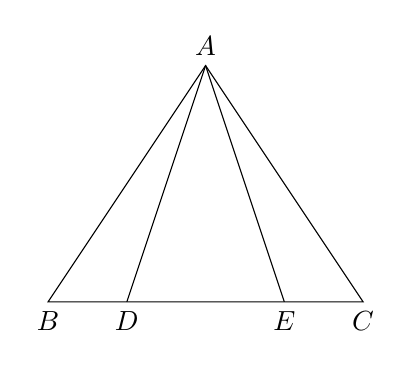
\begin{tikzpicture} 
%	\coordinate (A) at (2, 3) {};
%	\coordinate (B) at (0, 0) {};
%	\coordinate (C) at (4, 0) {};
%	\coordinate (D) at (1, 0) {};
%	\coordinate (E) at (3, 0) {};
%	\draw (A)node[above]{$A$}--(B)node[below]{$B$}--(C)node[below]{$C$}--cycle;
%	\draw (B)node[below]{}--(E)node[below]{$E$};
%	\draw (C)node[below]{}--(D)node[below]{$D$};
	
	
	
	\coordinate (A) at (2,3){};
	\coordinate (B) at (0, 0){};
	\coordinate (C) at (4, 0){};
	\coordinate (D) at (1, 0){};
	\coordinate (E) at (3, 0){};
	
	%Drawing triangle ABC
	\draw (A)node[above]{$A$}--(B)node[below]{$B$}--(C)node[below]{$C$}--cycle;
	\draw (A)node[above]{}--(D)node[below]{$D$};
	\draw (A)node[above]{}--(E)node[below]{$E$};
	
\end{tikzpicture}}
		\caption{Isosceles Triangle with sides AB = AC}
	\end{figure}
	We are given that the sides $AB = AC$, and $BE = CD$. These two can be represented as
	\begin{align}\label{eq:solutions/1/17/eq:fact1}
		\norm{\vec{B}-\vec{A}} = \norm{\vec{C}-\vec{A}}
	\end{align}
	\begin{align}\label{eq:solutions/1/17/eq:fact2}
		\norm{\vec{B}-\vec{E}} = \norm{\vec{D}-\vec{C}}
	\end{align}
	
	Since the given trianle is an isoceles triangle, the angles formed by $AB$ and $AC$ on $BC$ will be the same. That is
	\begin{align}\label{eq:solutions/1/17/eq:fact3}
		\angle ABC &= \angle ACB = \alpha
	\end{align}
	The side $AD$ can be represented as 
	\begin{align}\label{eq:solutions/1/17/eq:eq1}
		(\vec{D-A}) &= (\vec{B-A}) - (\vec{B-D})
	\end{align}
	Squaring both the sides we get	
	\begin{align} \label{eq:solutions/1/17/eq:eq2}
		\norm{\vec{D}-\vec{A}}^{2} = \norm{\vec{B}-\vec{A}}^{2} + \norm{\vec{B}-\vec{D}}^{2} \nonumber \\ - 2\norm{\vec{B}-\vec{A}}\norm{\vec{B}-\vec{D}}\cos\alpha
	\end{align}
	The side $AE$ can be represented as 
	\begin{align}\label{eq:solutions/1/17/eq:eq3}
		(\vec{A-E}) &= (\vec{C-A}) - (\vec{C-E})
	\end{align}
	Squaring both the sides we get	
	\begin{align} \label{eq:solutions/1/17/eq:eq4}
		\norm{\vec{A}-\vec{E}}^{2} = \norm{\vec{C}-\vec{A}}^{2} + \norm{\vec{C}-\vec{E}}^{2} \nonumber \\  - 2\norm{\vec{C}-\vec{A}}\norm{\vec{C}-\vec{E}}\cos\alpha
	\end{align}
	
	From \eqref{eq:solutions/1/17/eq:fact2}, we can further $(\vec{E-B})$ write it as 
	\begin{align}\label{eq:solutions/1/17/eq:eq5}
		(\vec{E-B}) &= (\vec{D-B}) + (\vec{E-D})
	\end{align}
	Squaring both the sides we get
	\begin{align} \label{eq:solutions/1/17/eq:eq6}
		\norm{\vec{E}-\vec{B}}^{2} = \norm{\vec{D}-\vec{B}}^{2} + \norm{\vec{E}-\vec{D}}^{2} \nonumber \\ + 2\norm{\vec{D}-\vec{B}}\norm{\vec{E}-\vec{D}}\cos\theta
	\end{align}
	Since, both the vectors are on the same direction, the angle between them is $\theta = 0\degree$.
	\begin{align} \label{eq:solutions/1/17/eq:eq7}
		\norm{\vec{E}-\vec{B}}^{2} = \norm{\vec{D}-\vec{B}}^{2} + \norm{\vec{E}-\vec{D}}^{2} \nonumber \\ + 2\norm{\vec{D}-\vec{B}}\norm{\vec{E}-\vec{D}}
	\end{align}
	\begin{align}\label{eq:solutions/1/17/eq:eq8}
		\norm{\vec{E}-\vec{B}}^{2} &= \left(\norm{\vec{D}-\vec{B}} + \norm{\vec{E}-\vec{D}}\right)^{2}
	\end{align}

	From \eqref{eq:solutions/1/17/eq:fact2}, we can further $(\vec{C-D})$ write it as
	\begin{align}\label{eq:solutions/1/17/eq:eq9}
		(\vec{C-D}) &= (\vec{C-E}) + (\vec{E-D})
	\end{align}
	Squaring both the sides we get
	\begin{align} \label{eq:solutions/1/17/eq:eq10}
		\norm{\vec{C}-\vec{D}}^{2} = \norm{\vec{C}-\vec{E}}^{2} + \norm{\vec{E}-\vec{D}}^{2} \nonumber \\ + 2\norm{\vec{C}-\vec{E}}\norm{\vec{E}-\vec{D}}\cos\theta
	\end{align}
	Since, both the vectors are on the same direction, the angle between them is $\theta = 0\degree$.
	\begin{align} \label{eq:solutions/1/17/eq:eq11}
		\norm{\vec{C}-\vec{D}}^{2} = \norm{\vec{C}-\vec{E}}^{2} + \norm{\vec{E}-\vec{D}}^{2} \nonumber \\ + 2\norm{\vec{C}-\vec{E}}\norm{\vec{E}-\vec{D}}
	\end{align}
	\begin{align}\label{eq:solutions/1/17/eq:eq12}
		\norm{\vec{C}-\vec{D}}^{2} &= \left(\norm{\vec{C}-\vec{E}} + \norm{\vec{E}-\vec{D}}\right)^{2}
	\end{align}

	From equations \eqref{eq:solutions/1/17/eq:fact2}, \eqref{eq:solutions/1/17/eq:eq8}, \eqref{eq:solutions/1/17/eq:eq12}, we get
	
	\begin{align}\label{eq:solutions/1/17/eq:eq13}
		\left(\norm{\vec{D}-\vec{B}} + \norm{\vec{E}-\vec{D}}\right)^{2} &= \left(\norm{\vec{C}-\vec{E}} + \norm{\vec{E}-\vec{D}}\right)^{2} \nonumber \\
		\implies \norm{\vec{D}-\vec{B}} + \norm{\vec{E}-\vec{D}} &= \norm{\vec{C}-\vec{E}} + \norm{\vec{E}-\vec{D}} \nonumber \\
		\implies \norm{\vec{D}-\vec{B}} &= \norm{\vec{C}-\vec{E}}
	\end{align}

	Using equations \eqref{eq:solutions/1/17/eq:fact1}, \eqref{eq:solutions/1/17/eq:eq13}, we apply them in the equation \eqref{eq:solutions/1/17/eq:eq2}, \eqref{eq:solutions/1/17/eq:eq4}. After applying it we see that the R.H.S components are getting equated to each other, then we can equate the L.H.S as well. We get 
	\begin{align}\label{eq:solutions/1/17/eq:eq15}
		\norm{\vec{D}-\vec{A}}^{2} &= \norm{\vec{A}-\vec{E}}^{2} \nonumber \\
		\norm{\vec{D}-\vec{A}} &= \norm{\vec{A}-\vec{E}}
	\end{align}
	
	Therefore, we can say that $AD = AE$.
	
